\documentclass{article}
\usepackage{amsmath}
\usepackage{graphicx}
\usepackage{xcolor}
\usepackage{listings}
\usepackage{geometry}
\usepackage{circuitikz}
\geometry{legalpaper, left=20mm,top=25mm}
\usepackage[utf8]{inputenc}
\renewcommand{\familydefault}{\sfdefault}
\renewcommand{\baselinestretch}{1.5}

\definecolor{numberingcolor}{rgb}{1,0,0}
\definecolor{backgroundcolour}{rgb}{0.97,0.97,0.97}

\lstdefinestyle{CodeStyle}{
  backgroundcolor=\color{backgroundcolour},
  numberstyle=\tiny\color{numberingcolor},
  basicstyle=\ttfamily\footnotesize,
  breakatwhitespace=false,         
  breaklines=false,                 
  captionpos=b,                    
  keepspaces=true,                 
  numbers=left,                    
  numbersep=5pt,                  
  showspaces=false,                
  showstringspaces=false,
  showtabs=false,                  
  tabsize=7
}
\lstset{style=CodeStyle}

\title{EE3113 Homework Assignment-2}
\author{Krishna Srikar Durbha}
\date{EE18BTECH11014}

\begin{document}
\maketitle
\vspace{0.05in}
\textbf{Note:} Mathematical Explanations for some of the questions are at the end. 

\section{1.MOSFET Resistance}
\textbf{Specifications:}
\begin{align}
    \frac{W}{L} = 240/180\\
    W = 240nm, L = 180nm\\
    V_{DD} = 1.8 \text{ Volts}, C = 1pF\\
    \text{Voltage Drop across on Capacitor = $1.8$ Volts} \\
    R = dV_{DS}/dI_D
\end{align}
\subsection{1a}
\subsubsection{N-MOSFET}
\textbf{SPICE Netlist}:
\begin{lstlisting}
Question-1 for N-MOSFET

* Model
.include "TSMC180.lib"
.model nch_tt nmos

* Circuit
Vdd	G	0	DC	1.8	
V	1	D	DC	0
M	D	G	0	0	nch_tt W=240n L=180n
C	1	0	1p

* Analysis
.tran	0.1p	50n

* Results
.ic	V(1) = 1.8
.control
run
let ID = V#branch
plot	ID vs V(D)
plot	V(D)/ID vs V(D)
.endc

.end
\end{lstlisting}
\pagebreak
\textbf{Results:}
\begin{figure}[!ht]
    \centering
    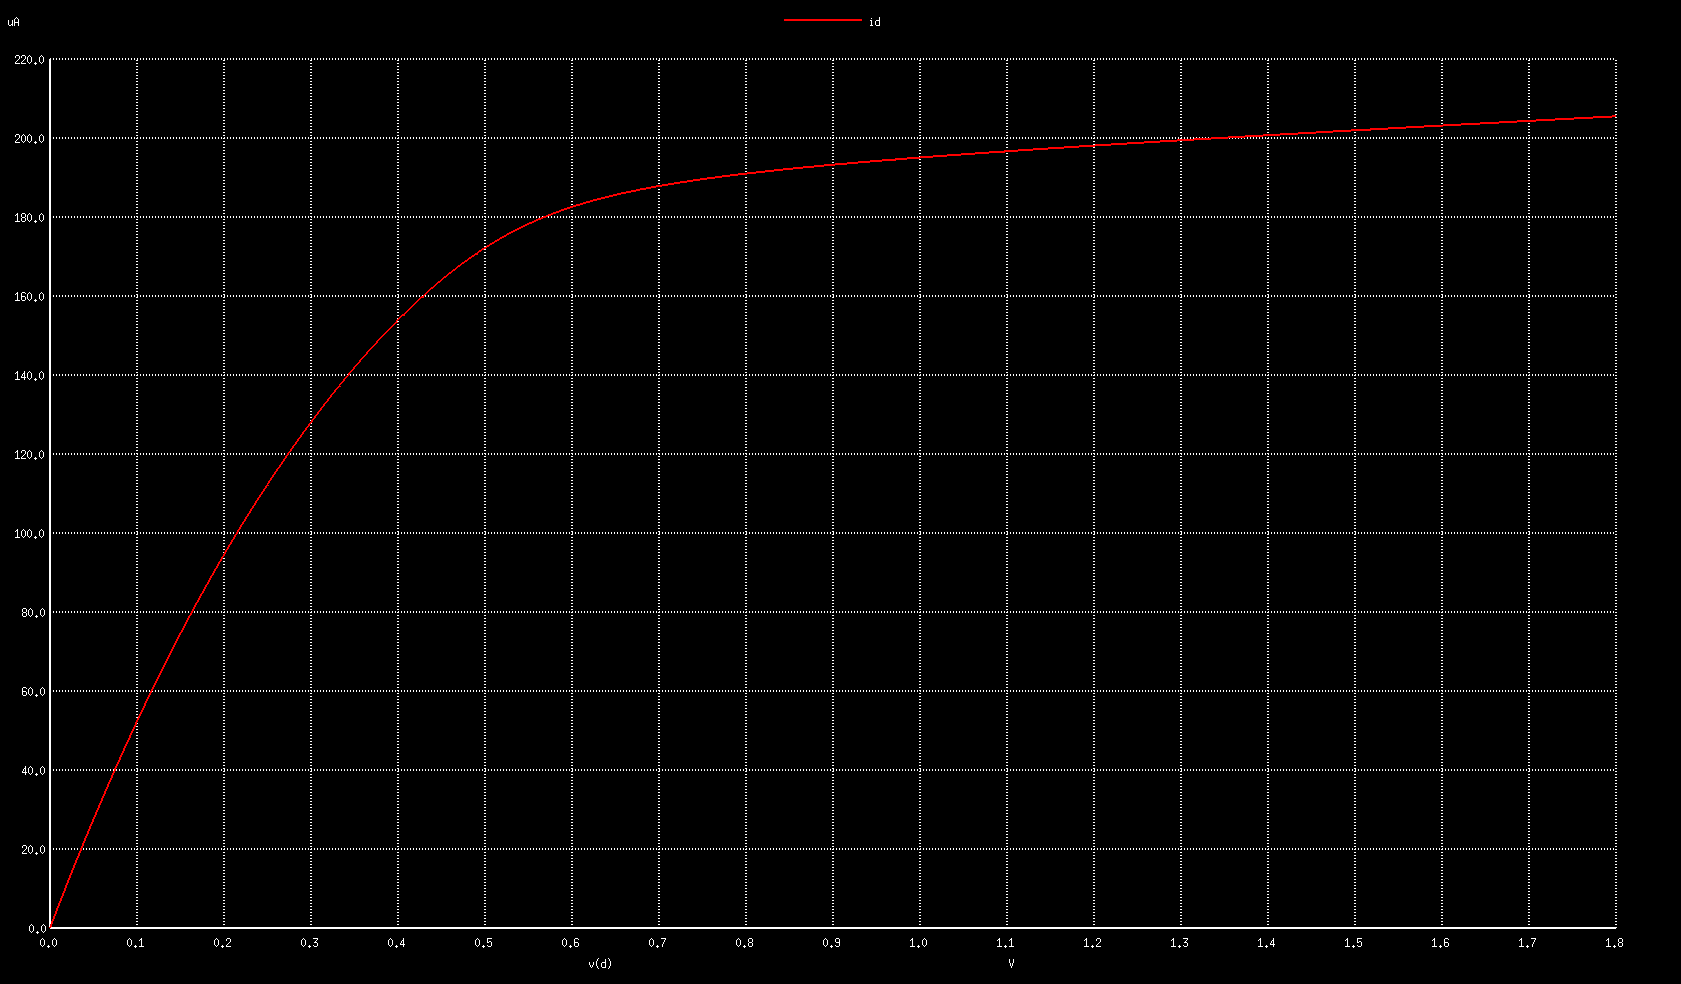
\includegraphics[scale=0.23]{Images/1nmosa.png}
    \caption{$I_D$ vs $V_{DS}$ Characteristics of N-MOSFET}
\end{figure}
\begin{figure}[!ht]
    \centering
    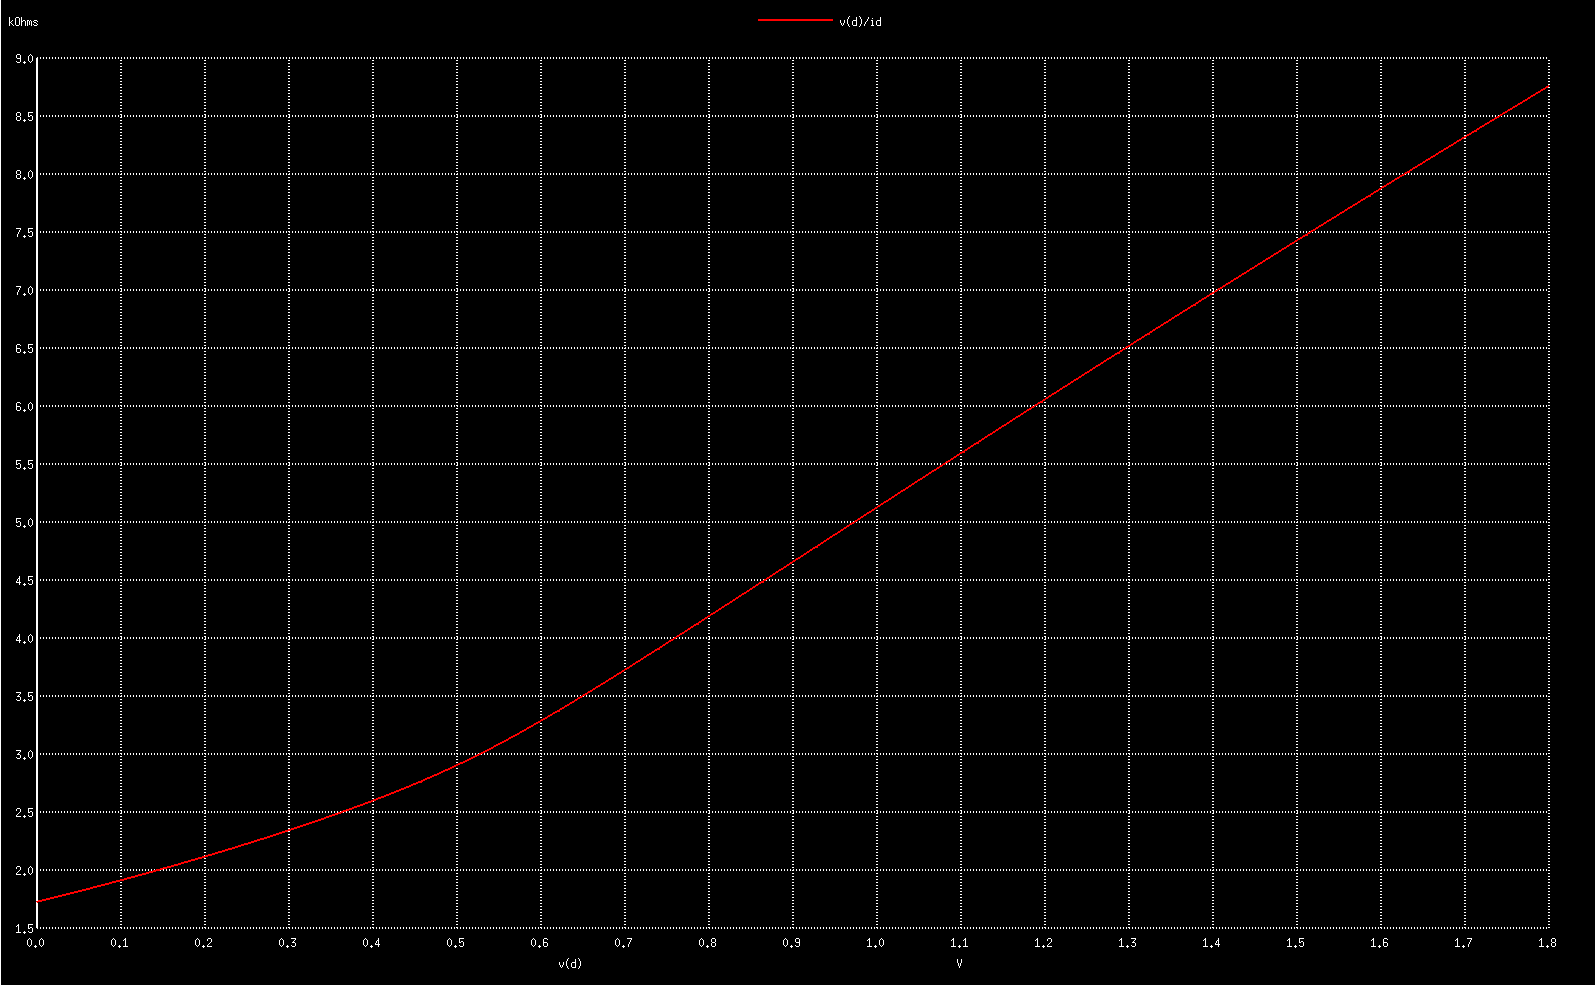
\includegraphics[scale=0.24]{Images/1nmosb.png}
    \caption{$R$ vs $V_{DS}$ Characteristics of N-MOSFET}
\end{figure}

\subsubsection{P-MOSFET}
\textbf{SPICE Netlist}:
\begin{lstlisting}
Question-1 for P-MOSFET

* Model
.include "TSMC180.lib"
.model pch_tt pmos

* Circuit
Vdd	G	0	DC	-1.8	
V	1	D	DC	0
M	D	G	0	0	pch_tt W=240n L=180n
C	1	0	1p

* Analysis
.tran	0.1p	50n

* Results
.ic	V(1) = -1.8
.control
run
let ID = V#branch 
plot	ID vs V(D)
plot	V(D)/ID vs V(D)
.endc

.end
\end{lstlisting}
\textbf{Results:}
\begin{figure}[!ht]
    \centering
    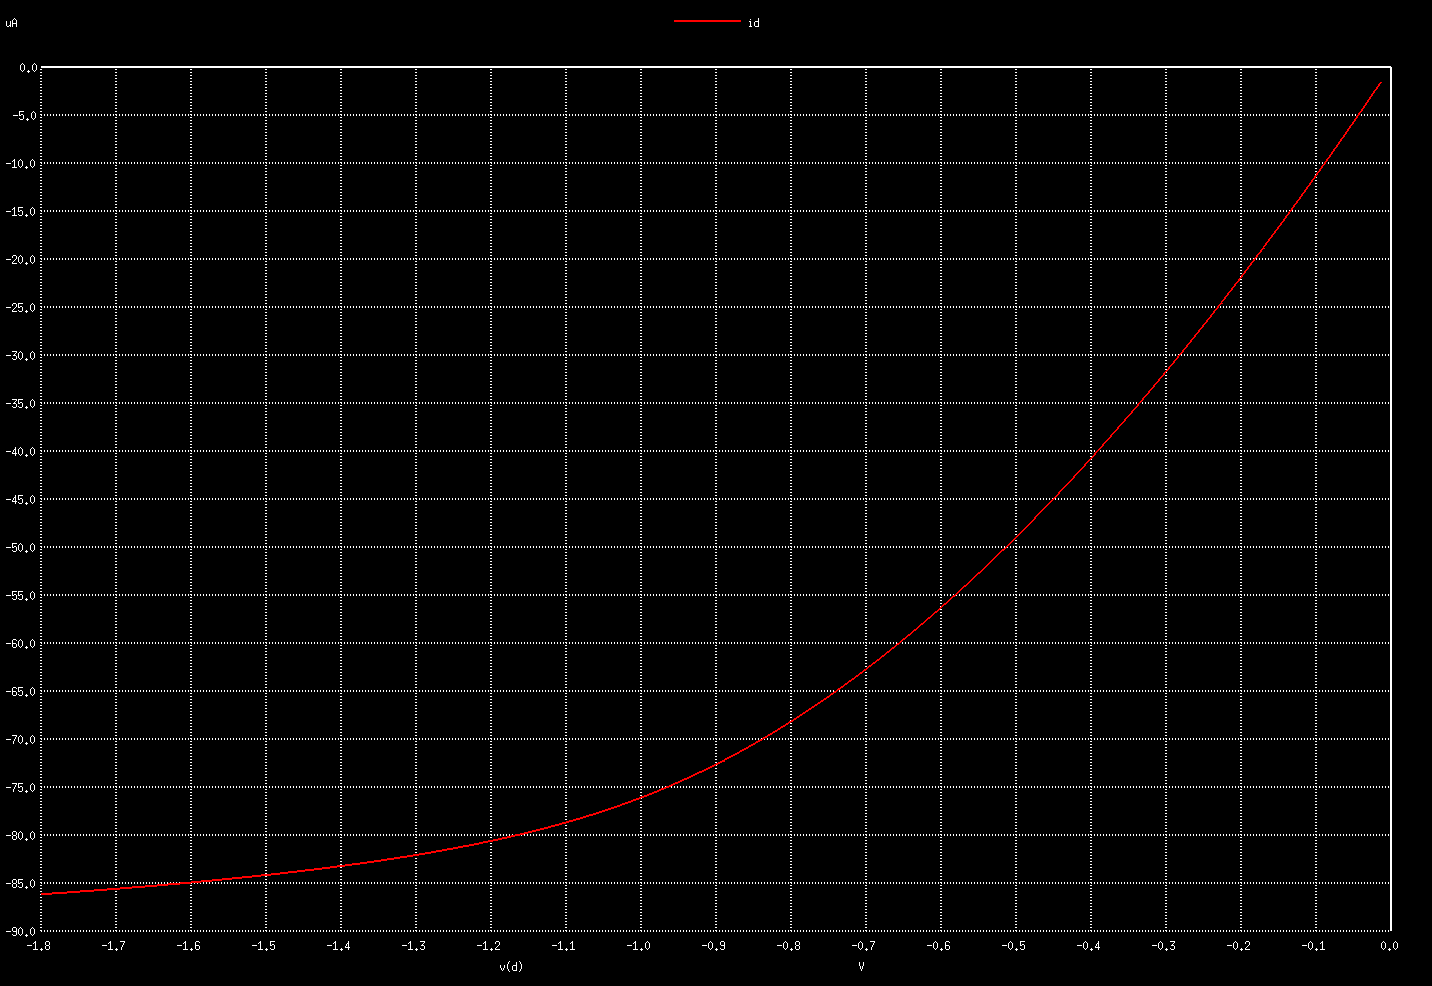
\includegraphics[scale=0.25]{Images/1pmosa.png}
    \caption{$I_D$ vs $V_{DS}$ Characteristics of P-MOSFET}
\end{figure}
\begin{figure}[!ht]
    \centering
    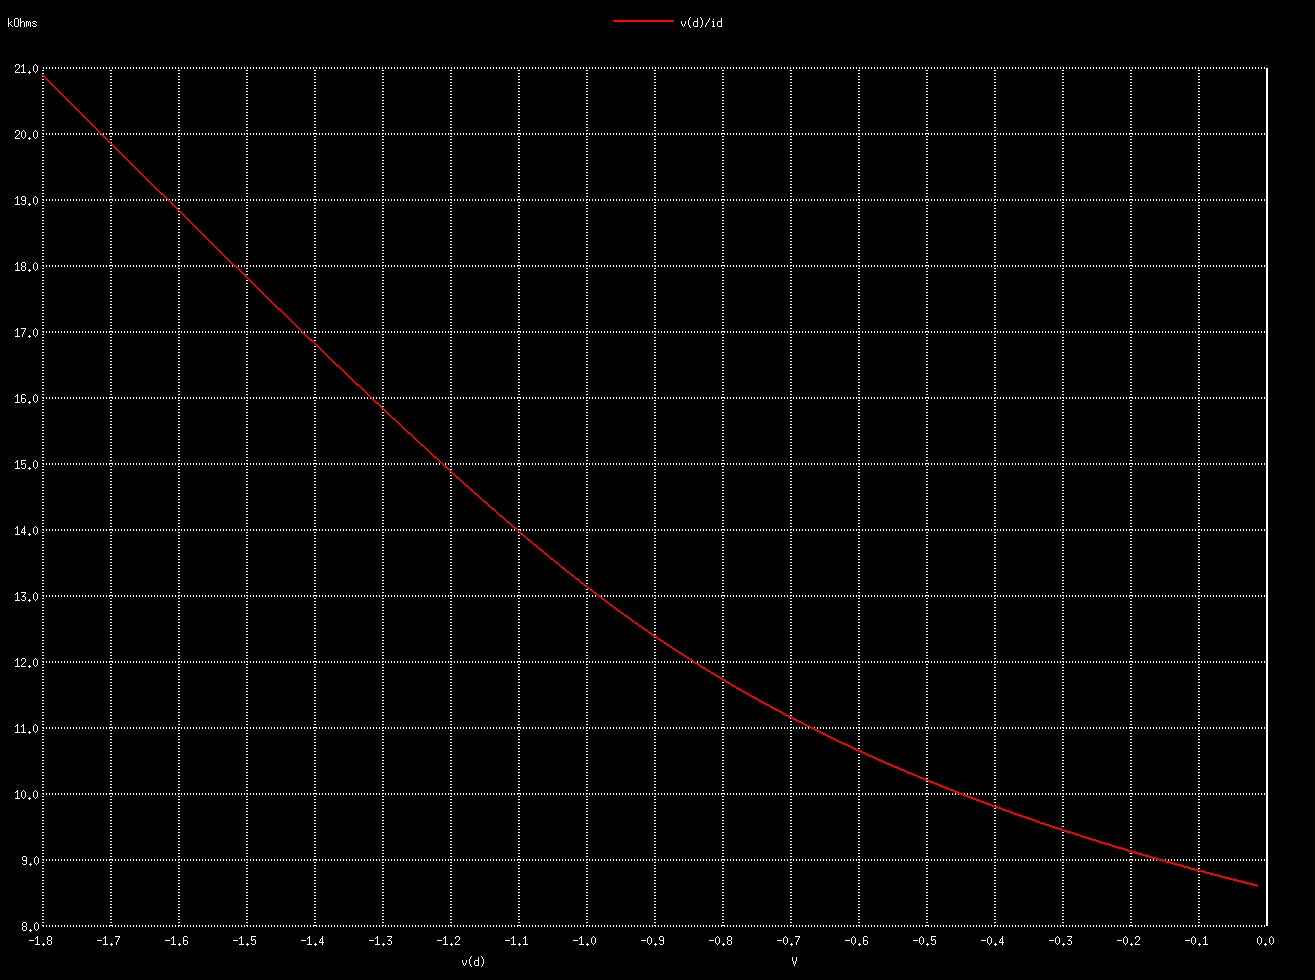
\includegraphics[scale=0.27]{Images/1pmosb.png}
    \caption{$R$ vs $V_{DS}$ Characteristics of P-MOSFET}
\end{figure}

\subsection{1b}
\begin{align}
    R_{eq} = 0.5\times\left[R(V_{DS} = \frac{V_{DD}}{2}) + R(V_{DS} = V_{DD})\right]
\end{align}
\subsubsection{N-MOSFET}
\begin{center}
    \begin{tabular}{ |p{3cm}|p{4cm}|p{4cm}|p{3cm}| } 
    \hline
    $V_{GS}$ (in Volts) & $R\left(V_{DS} = 0.5V_{DD}\right)$ (in $\Omega$) & $R\left(V_{DS} = V_{DD}\right)$ (in $\Omega$) & $R_{eq}$ (in $\Omega$)\\ 
    \hline
    \hline
    1.8 & 4660 & 8772.73 & 6616.4\\
    \hline
    1.5 & 5235.29 & 9803.92 & 7519.605\\
    \hline
    1.2 & 6463.67 & 12063.3 & 9263.485\\
    \hline
    0.9 & 10320 & 18620 & 14470\\
    \hline
    0.6 & 47070.7 & 80000 & 63535.35\\
    \hline
    \end{tabular}
\end{center}
\vspace{0.1in}
\subsubsection{P-MOSFET}
\begin{center}
    \begin{tabular}{ |p{3cm}|p{4cm}|p{4cm}|p{3cm}| } 
    \hline
    $V_{GS}$ (in Volts) & $R\left(V_{DS} = 0.5V_{DD}\right)$ (in $\Omega$) & $R\left(V_{DS} = V_{DD}\right)$ (in $\Omega$) & $R_{eq}$ (in $\Omega$)\\ 
    \hline
    \hline
    -1.8 & 12393.9 & 20878.8 & 16636.35\\
    \hline
    -1.5 & 16062.5 & 27541.7 & 21802.1\\
    \hline
    -1.2 & 23762.7 & 41355.9 & 32559.3\\
    \hline
    -0.9 & 44793.8 & 79278.4 & 62036.1\\
    \hline
    -0.6 & 178958 & 321277 & 250117.5\\
    \hline
    \end{tabular}
\end{center}
There is a huge difference between values in **Table 3.3** of Reference Book and our Values, is because of the $\frac{W}{L}$ ratio between the MOSFETs. 
\pagebreak
\section{2.MOSFET Capacitance}
\begin{figure}[!ht]
    \centering
    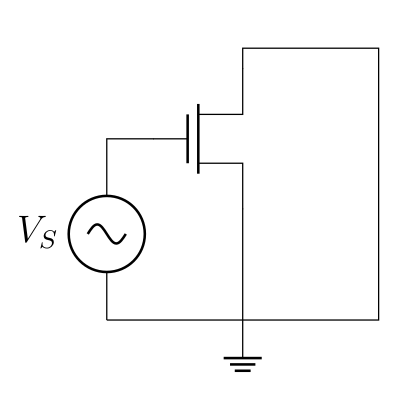
\includegraphics[scale=0.5]{Images/2.png}
\end{figure}
\textbf{Specifications for Short Channel MOSFET:}
\begin{align}
    L = 180 \text{ nm} \\
    W = 450 \text{ nm}
\end{align}
\vspace{0.2in}
\textbf{Specifications for Long Channel MOSFET:}
\begin{align}
    L = 10 \text{ $\mu$m} \\
    W = 25 \text{ $\mu$m}
\end{align}
\vspace{0.2in}
\textbf{Calculations:}
\begin{align}
    V_{applied} = V_{CM} + V_{0}\sin(\omega t)  \\
    V_{0} = \frac{1}{2\pi f} = \frac{1}{\omega} \\
    I = CV_{0}\omega\cos(\omega t) = C\cos(\omega t) \\
    C = I(t=\frac{2\pi}{\omega})
\end{align}
For plotting Gate Capacitance vs $V_{GS}$, $V_{GS} = V_{CM}$ is varied from $[-1.8,1.8]$ Volts.
\vspace{0.2in}
\subsection{2a}
Assuming,
\begin{align}
    f = 100 \text{ Hz} \\
    V_{0} = \frac{1}{2\pi f} = 0.00159154943 \text{ Volts}\\
    V_{0} \approx 0.0016 \text{ Volts}
\end{align}
\pagebreak
\subsubsection{Long Channel N-MOSFET}
\textbf{SPICE Netlist:}
\begin{lstlisting}
Question-2a Long Channel N-MOSFET

* Model
.include "TSMC180.lib"
.model nch_tt nmos

* Circuit
Vs	G	1	AC	SIN(0 0.00159154943 100)
Vcm	1	0	DC	-1.8
M	0	G	0	0	nch_tt W=25u L=10u

* Results
.control
run

let Vg = -1.8
let X = vector(180)
let Y = vector(180)

while Vg < 1.81
	alter @Vcm Vg
	tran	10u	10m
	meas	tran	Capacitance	FIND	Vs#branch	AT = 10m
	let X[50*(Vg+1.8)] = Vg
	let Y[50*(Vg+1.8)] = -Capacitance

	let Vg = Vg + 0.02
end
plot	Y vs X

.endc
.end
\end{lstlisting}
\subsubsection{Short Channel N-MOSFET}
\textbf{SPICE Netlist:}
\begin{lstlisting}
Question-2a Short Channel N-MOSFET

* Model
.include "TSMC180.lib"
.model nch_tt nmos

* Circuit
Vs	G	1	AC	SIN(0 0.00159154943 100)
Vcm	1	0	DC	-1.8
M	0	G	0	0	nch_tt W=450n L=180n

* Results
.control
run

let Vg = -1.8
let X = vector(180)
let Y = vector(180)

while Vg < 1.81
	alter @Vcm Vg
	tran	10u	10m
	meas	tran	Capacitance	FIND	Vs#branch	AT = 10m
	let X[50*(Vg+1.8)] = Vg
	let Y[50*(Vg+1.8)] = -Capacitance

	let Vg = Vg + 0.02
end
plot	Y vs X

.endc
.end
\end{lstlisting}
\textbf{Results:}
\begin{figure}[!ht]
    \centering
    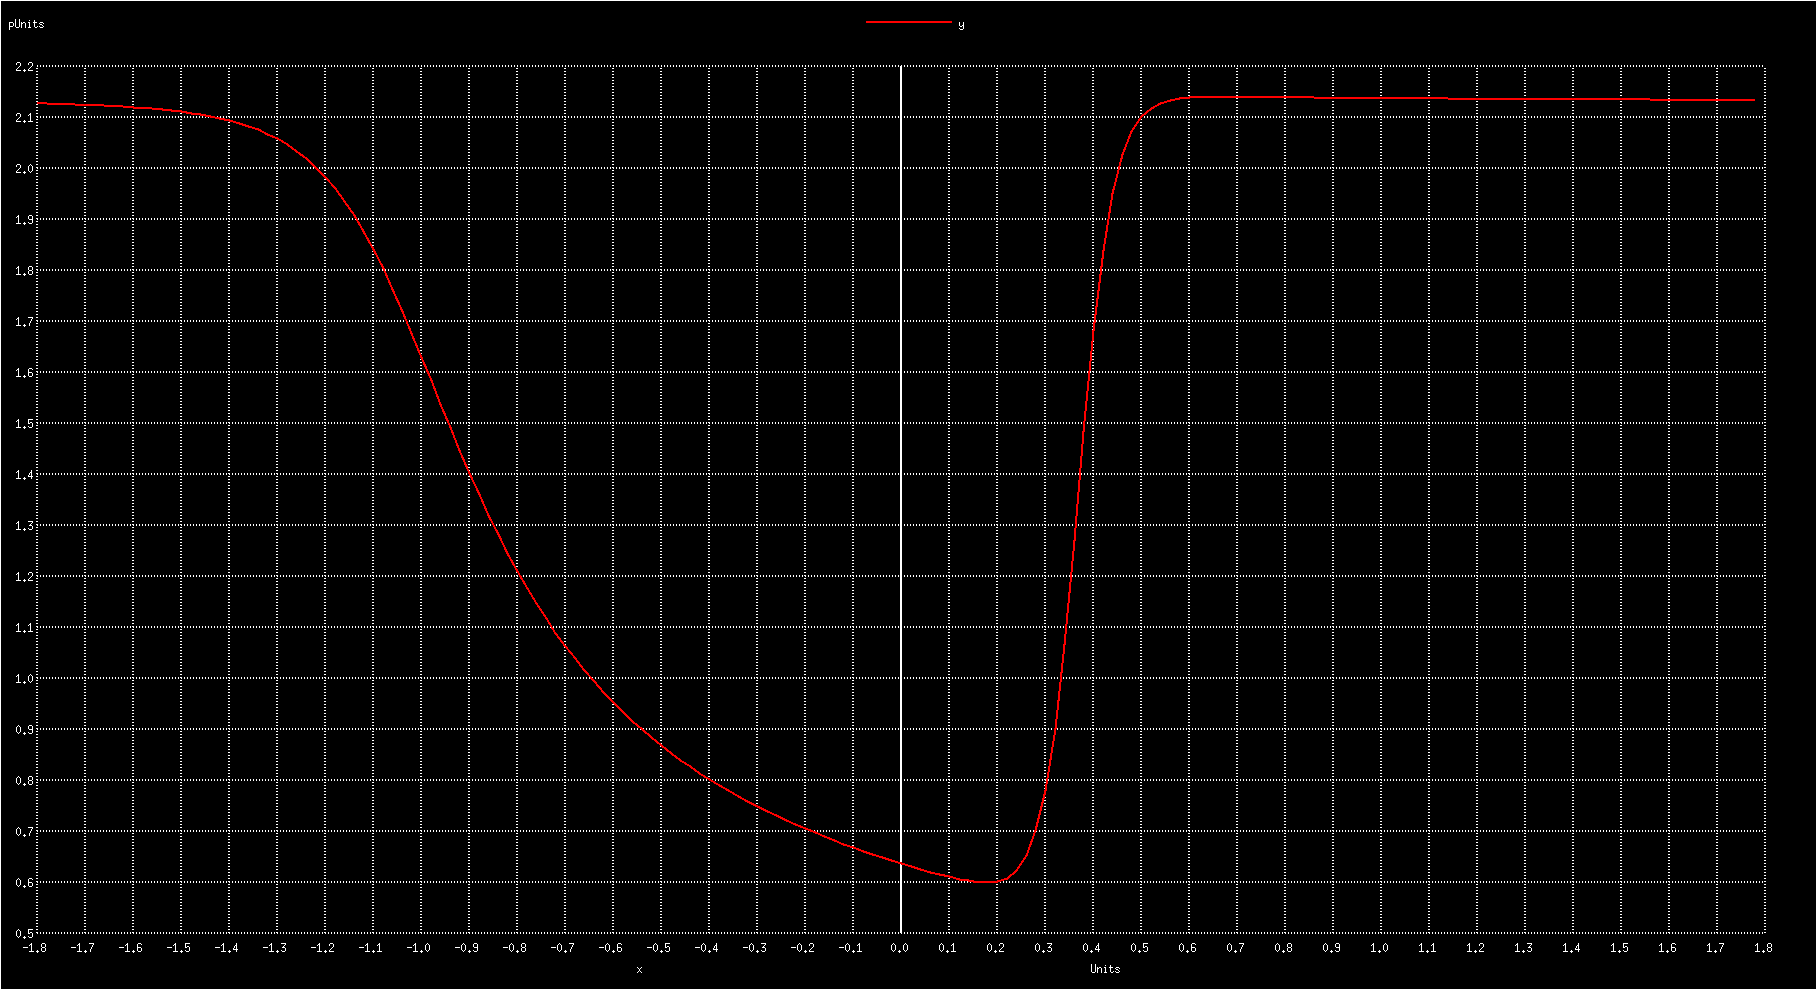
\includegraphics[scale=0.25]{Images/2along.png}
    \caption{$C$ vs $V_G$ for Long Channel Device}
\end{figure}
\begin{figure}[!ht]
    \centering
    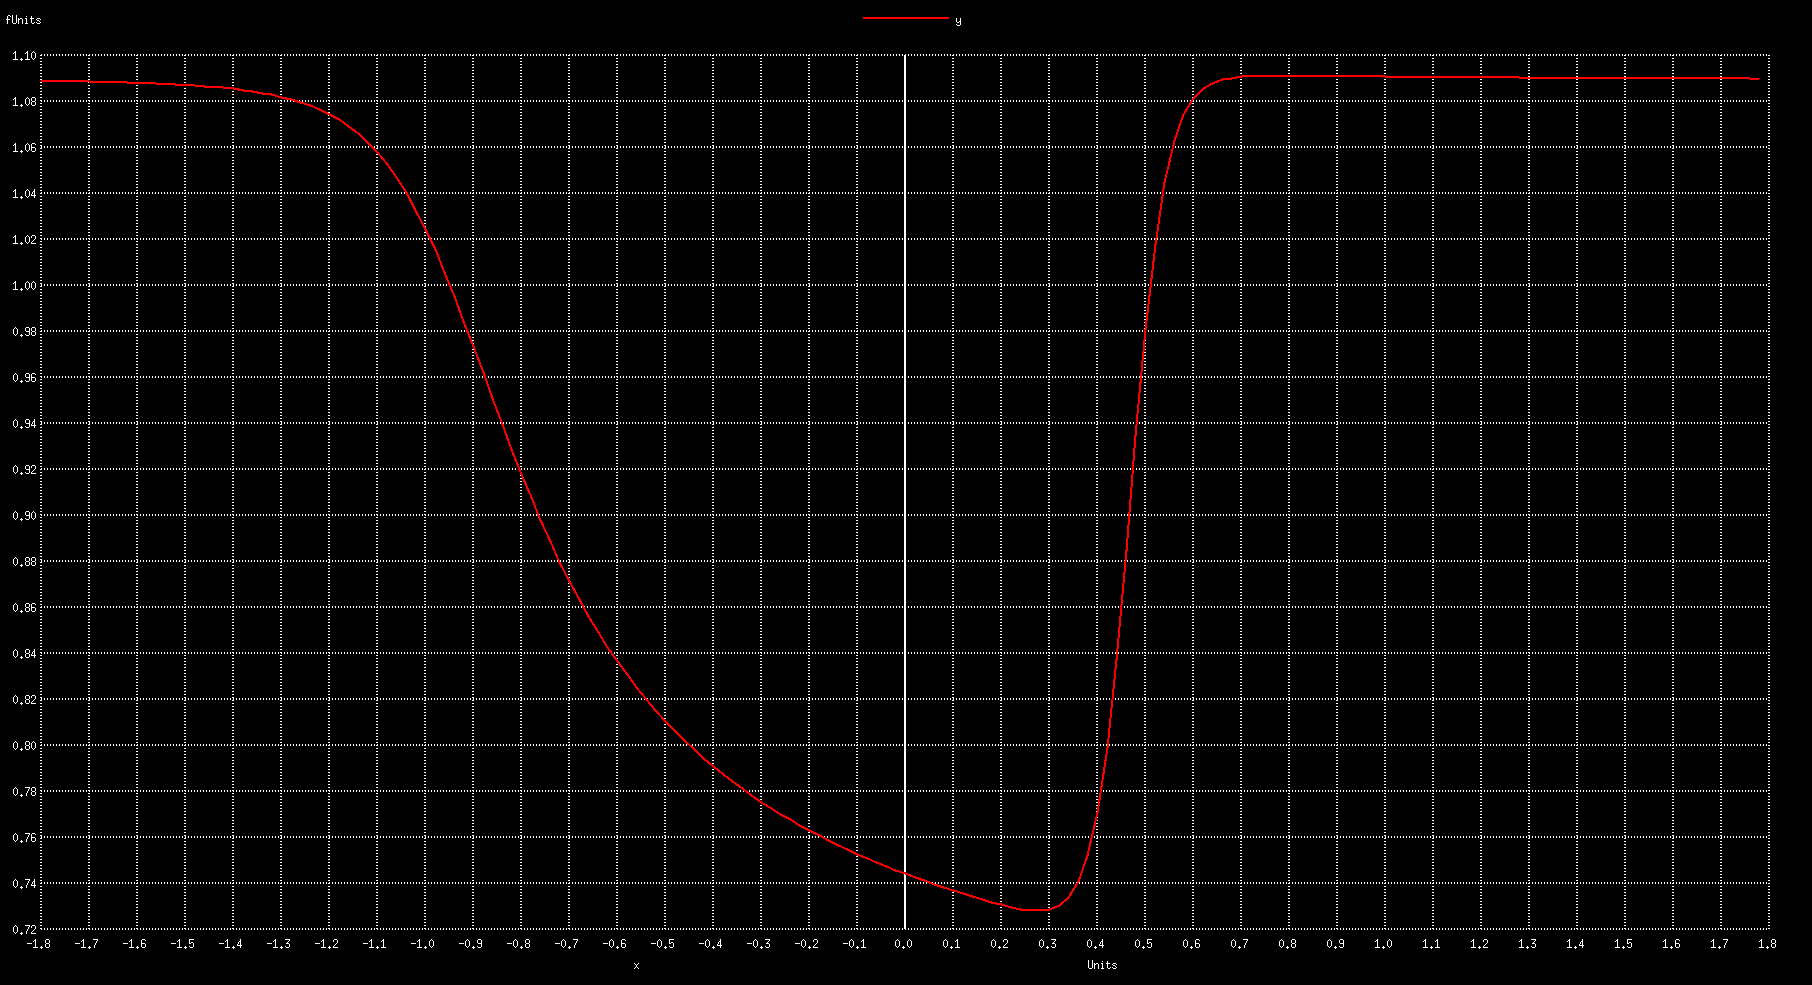
\includegraphics[scale=0.25]{Images/2ashort.png}
    \caption{$C$ vs $V_G$ for Short Channel Device}
\end{figure}
\subsection{2b}
\subsubsection{Long Channel N-MOSFET for f=10MHz}
\textbf{SPICE Netlist}
\begin{lstlisting}
Question-2b Long Channel N-MOSFET for f = 10MEG Hz

* Model
.include "TSMC180.lib"
.model nch_tt nmos

* Circuit
Vs	G	1	AC	SIN(0 0.000000015915 10MEG)
Vcm	1	0	DC	-1.8
M	0	G	0	0	nch_tt W=25u L=10u

* Results
.control
run

let Vg = -1.8
let X = vector(180)
let Y = vector(180)

while Vg < 1.81
	alter @Vcm Vg
	tran	1n	0.1u		
	meas	tran	Capacitance	FIND	Vs#branch	AT = 0.1u
	let X[50*(Vg+1.8)] = Vg
	let Y[50*(Vg+1.8)] = -Capacitance

	let Vg = Vg + 0.02
end
plot	Y vs X

.endc
.end
\end{lstlisting}
\textbf{Results:}
\begin{figure}[!ht]
    \centering
    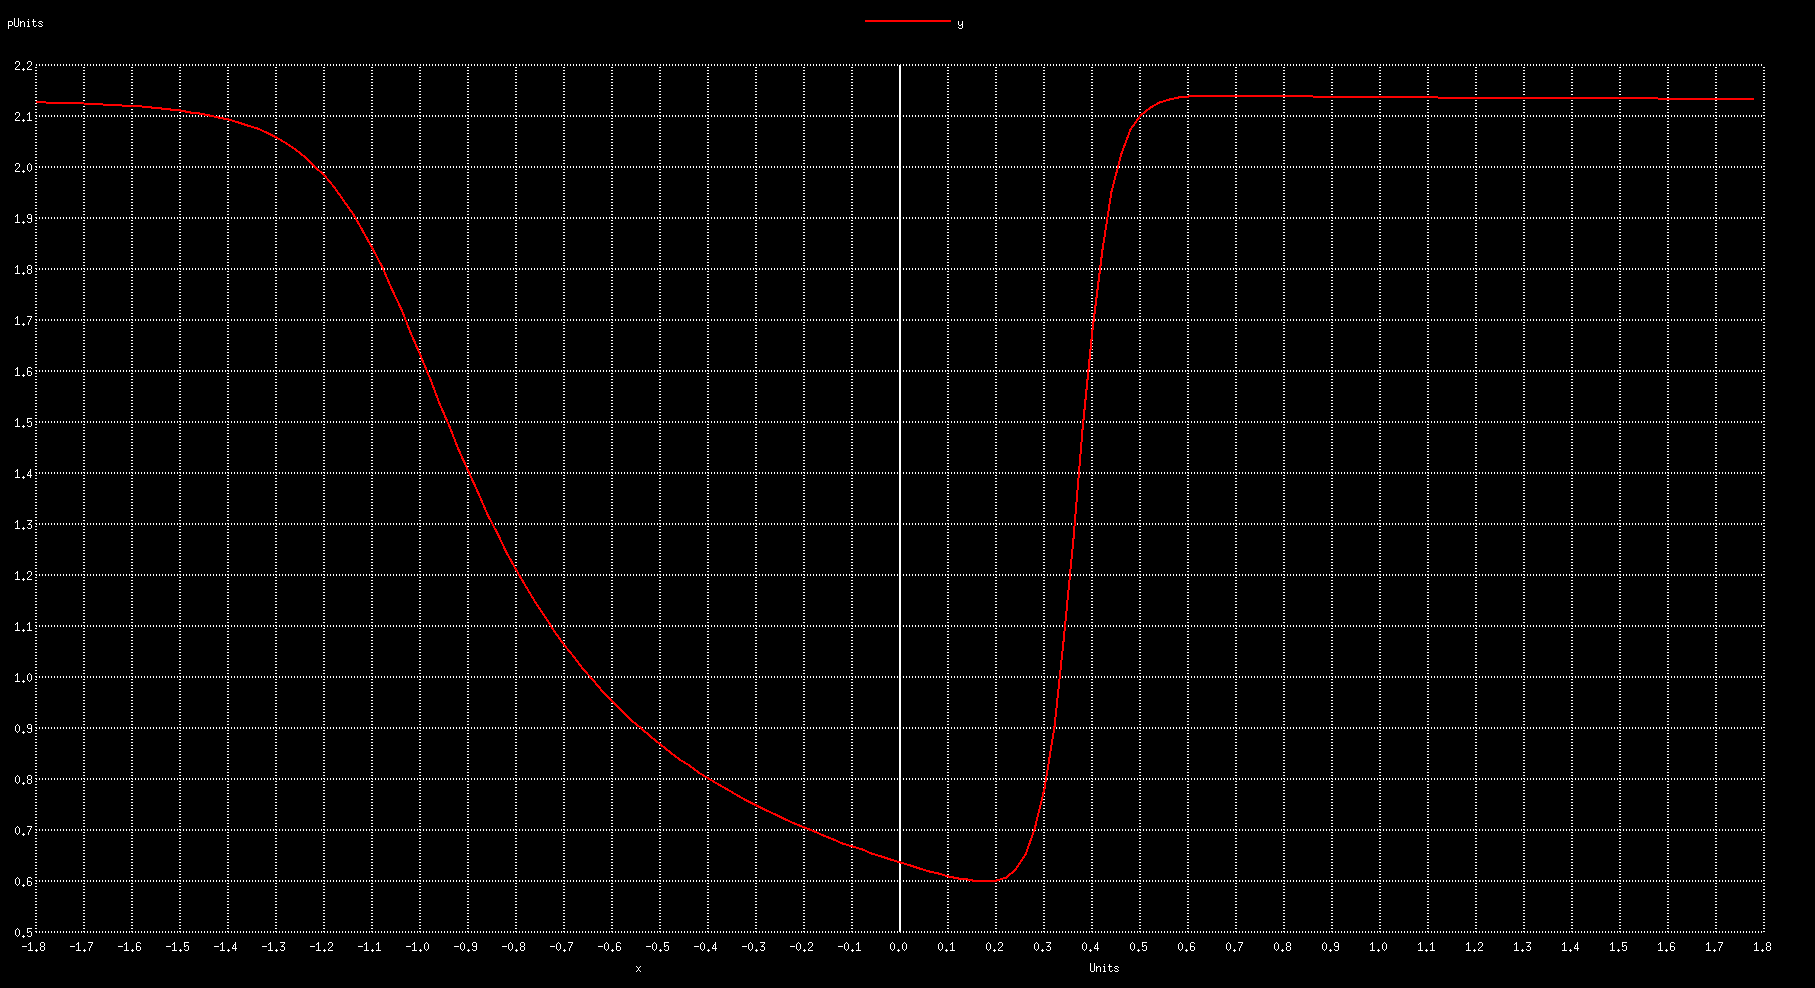
\includegraphics[scale=0.23]{Images/2blong1.png}
    \caption{$C$ vs $V_G$ for Long Channel Device for $f=10M$Hz}
\end{figure}

\subsubsection{Short Channel N-MOSFET for f=10MHz}
\textbf{SPICE Netlist}
\begin{lstlisting}
Question-2b Short Channel N-MOSFET for f = 10MEG Hz

* Model
.include "TSMC180.lib"
.model nch_tt nmos

* Circuit
Vs	G	1	AC	SIN(0 0.000000015915 10MEG)
Vcm	1	0	DC	-1.8
M	0	G	0	0	nch_tt W=450n L=180n

* Results
.control
run

let Vg = -1.8
let X = vector(180)
let Y = vector(180)

while Vg < 1.81
	alter @Vcm Vg
	tran	1n	0.1u		
	meas	tran	Capacitance	FIND	Vs#branch	AT = 0.1u
	let X[50*(Vg+1.8)] = Vg
	let Y[50*(Vg+1.8)] = -Capacitance

	let Vg = Vg + 0.02
end
plot	Y vs X

.endc
.end
\end{lstlisting}
\textbf{Results:}
\begin{figure}[!ht]
    \centering
    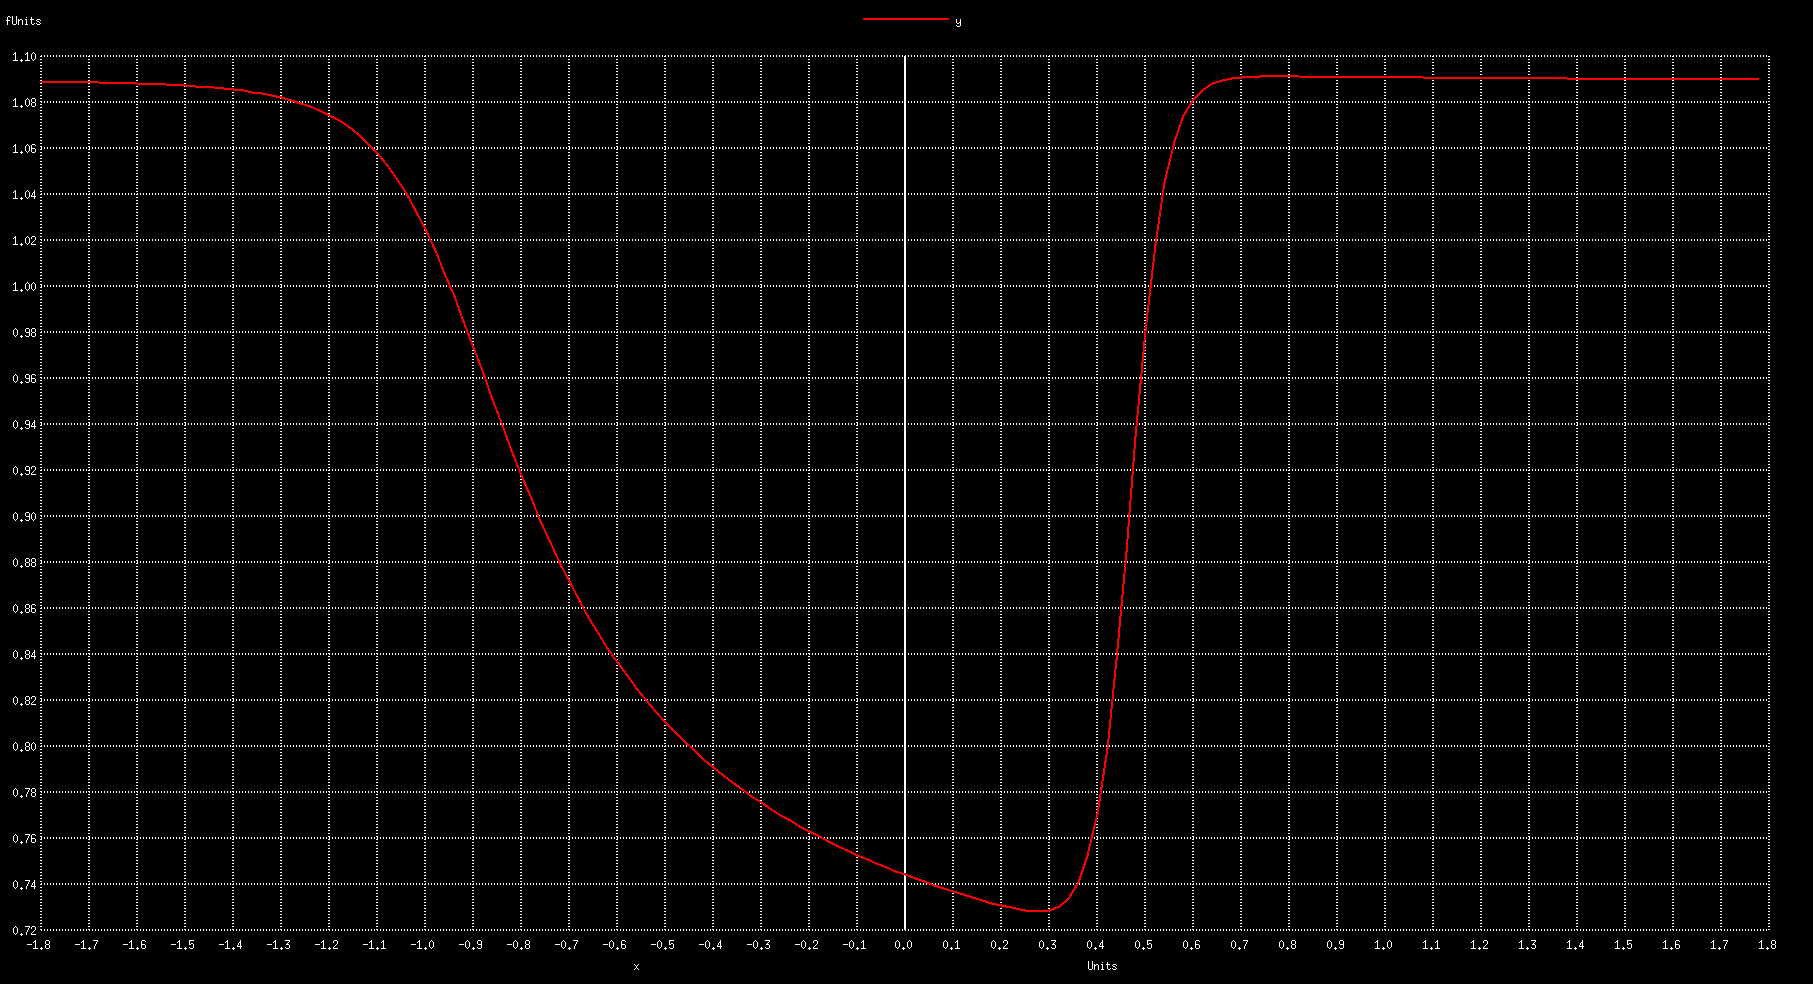
\includegraphics[scale=0.24]{Images/2bshort1.png}
    \caption{$C$ vs $V_G$ for Short Channel Device for $f=10M$Hz}
\end{figure}
\subsubsection{Long Channel N-MOSFET for f=10GHz}
\textbf{SPICE Netlist:}
\begin{lstlisting}
Question-2b Long Channel N-MOSFET for f = 10G Hz

* Model
.include "TSMC180.lib"
.model nch_tt nmos

* Circuit
Vs	G	1	AC	SIN(0 0.000000000015915 10G)
Vcm	1	0	DC	-1.8
M	0	G	0	0	nch_tt W=25u L=10u

* Results
.control
run

let Vg = -1.8
let X = vector(180)
let Y = vector(180)

while Vg < 1.81
	alter @Vcm Vg
	tran	5p	10.1n		
	meas	tran	Capacitance	FIND	Vs#branch	AT = 10n
	let X[50*(Vg+1.8)] = Vg
	let Y[50*(Vg+1.8)] = -Capacitance

	let Vg = Vg + 0.02
end
plot	Y vs X

.endc
.end
\end{lstlisting}
\textbf{Results:}
\begin{figure}[!ht]
    \centering
    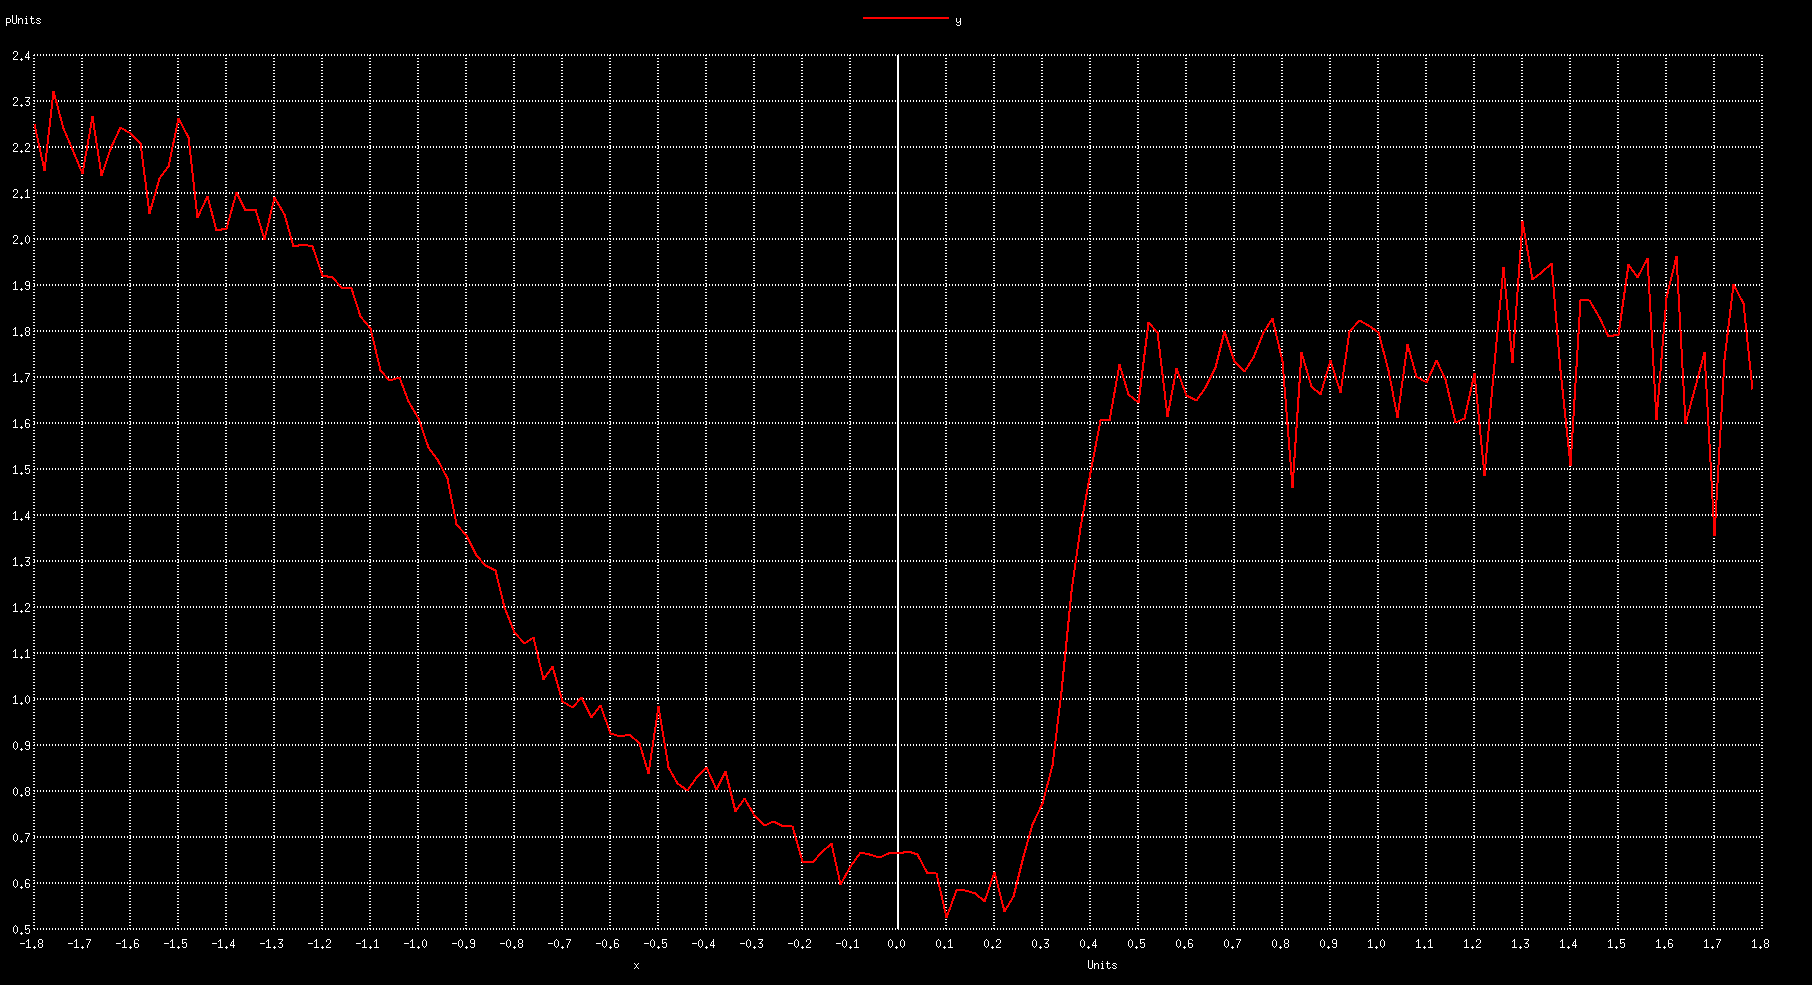
\includegraphics[scale=0.25]{Images/2blong2.png}
\end{figure}
\subsubsection{Short N-MOSFET for f=10GHz}
\textbf{SPICE Netlist:}
\begin{lstlisting}
Question-2b Short Channel N-MOSFET for f = 10G Hz

* Model
.include "TSMC180.lib"
.model nch_tt nmos

* Circuit
Vs	G	1	AC	SIN(0 0.000000000015915 10G)
Vcm	1	0	DC	-1.8
M	0	G	0	0	nch_tt W=450n L=180n

* Results
.control
run

let Vg = -1.8
let X = vector(180)
let Y = vector(180)

while Vg < 1.81
	alter @Vcm Vg
	tran	1p	0.101n		
	meas	tran	Capacitance	FIND	Vs#branch	AT = 0.1n
	let X[50*(Vg+1.8)] = Vg
	let Y[50*(Vg+1.8)] = -Capacitance

	let Vg = Vg + 0.02
end
plot	Y vs X

.endc
.end
\end{lstlisting}
\textbf{Results:}
\begin{figure}[!ht]
    \centering
    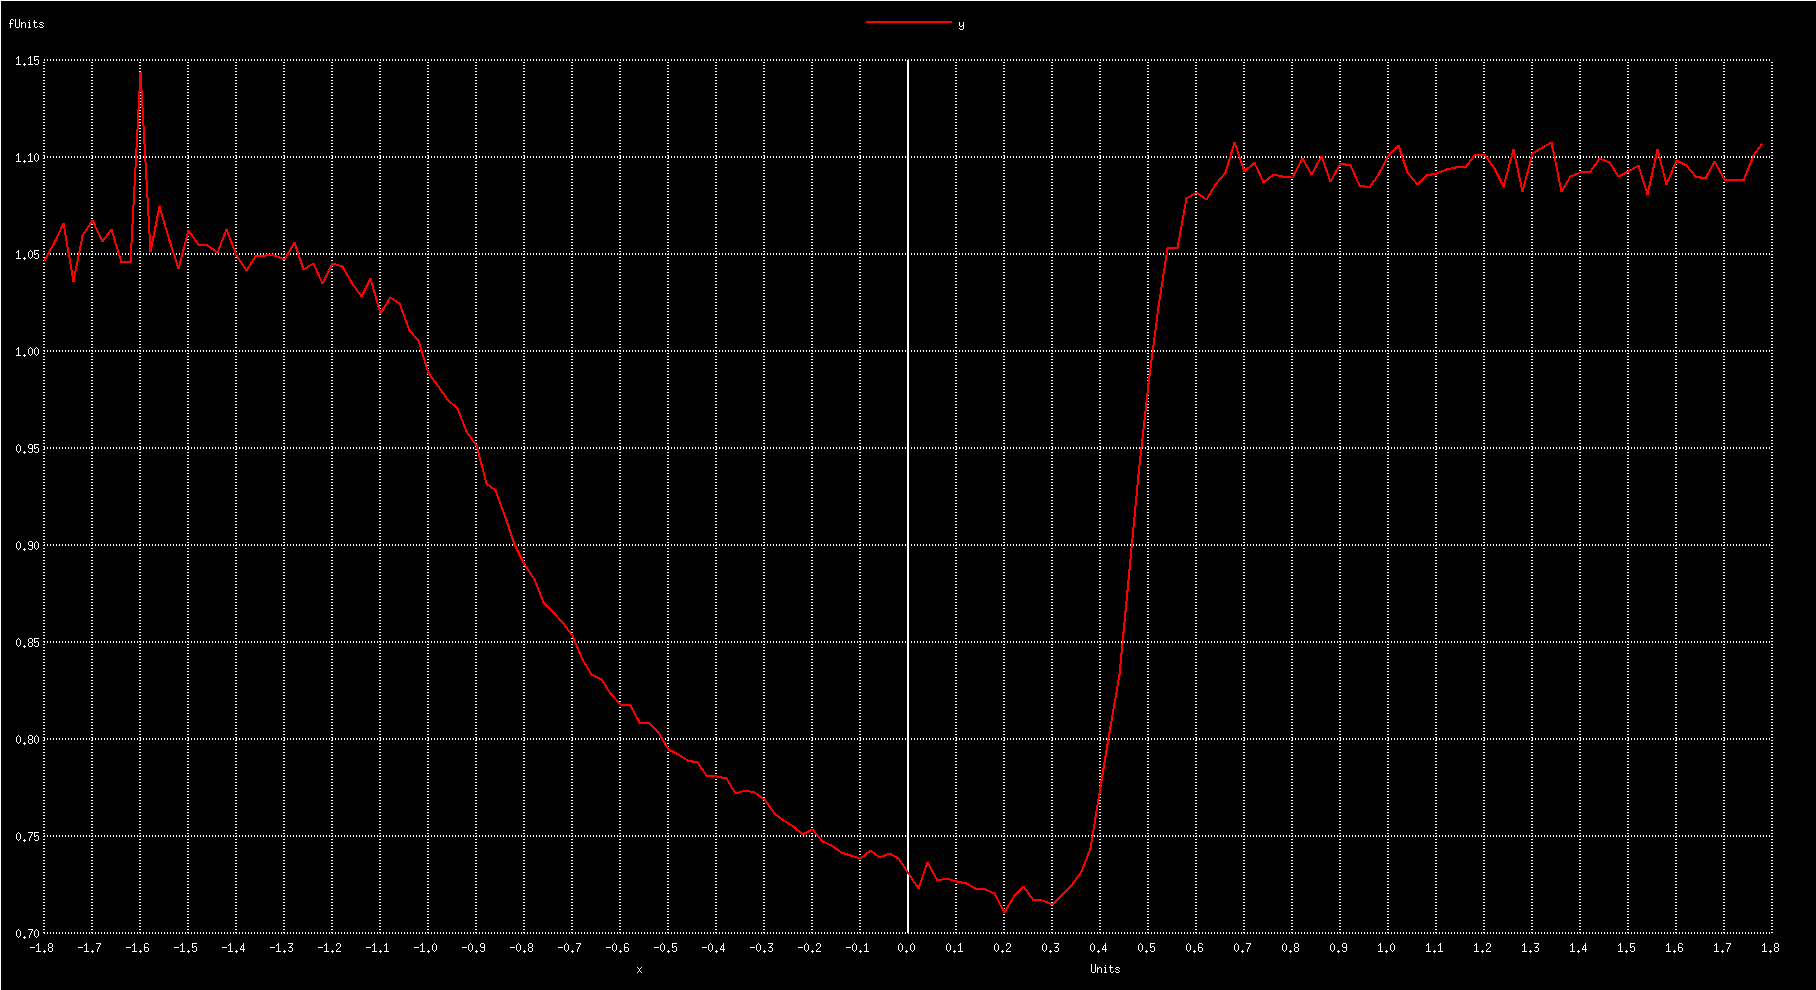
\includegraphics[scale=0.22]{Images/2bshort2.png}
\end{figure}\\
The difference between HFCV and LFCV characteristics is due to the time required for electrons to settle down. When the Frequency is high, there won't be be anytime for electrons to reach Gate end of MOSFET. When Frequency is Low, Electrons reach the Gate end and Capacitance increases.
\section{5.NMOS Inverter - SPICE simulations}
\begin{figure}[!ht]
    \centering
    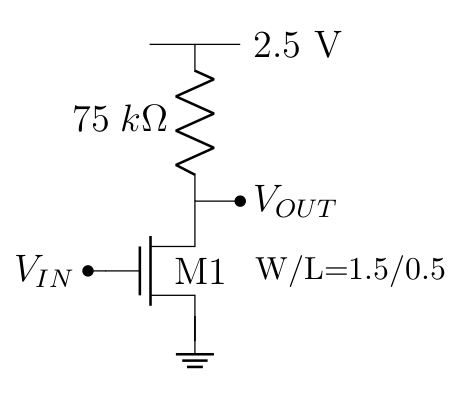
\includegraphics[scale=0.5]{Images/5a.png}
\end{figure}
\textbf{Specifications}
\begin{align}
    \frac{W}{L} = 1.5/0.5\\
    W = 540nm, L = 180nm\\
    V_{G} = [0,1.8] \text{ Volts}\\
    R = dI_D/dV_{DS}
\end{align}
\subsection{5a}
\textbf{SPICE Netlist}
\begin{lstlisting}
Question-5a

* Model
.include "TSMC180.lib"
.model nch_tt nmos

* Circuit
VG	G	0	1.8
M	D	G	0	0	nch_tt W=540n L=180n
R	D	2	75k
V	2	0	DC	2.5

* Analysis
.dc VG 0 1.8 1m

* Results
.control
run 
let ID = -V#branch
let Vout = V(D)
let Vin = V(G)
plot	Vout
plot	deriv(Vout)
.endc

.end
\end{lstlisting}
\pagebreak
\textbf{Results:}\\
\begin{figure}[!ht]
    \centering
    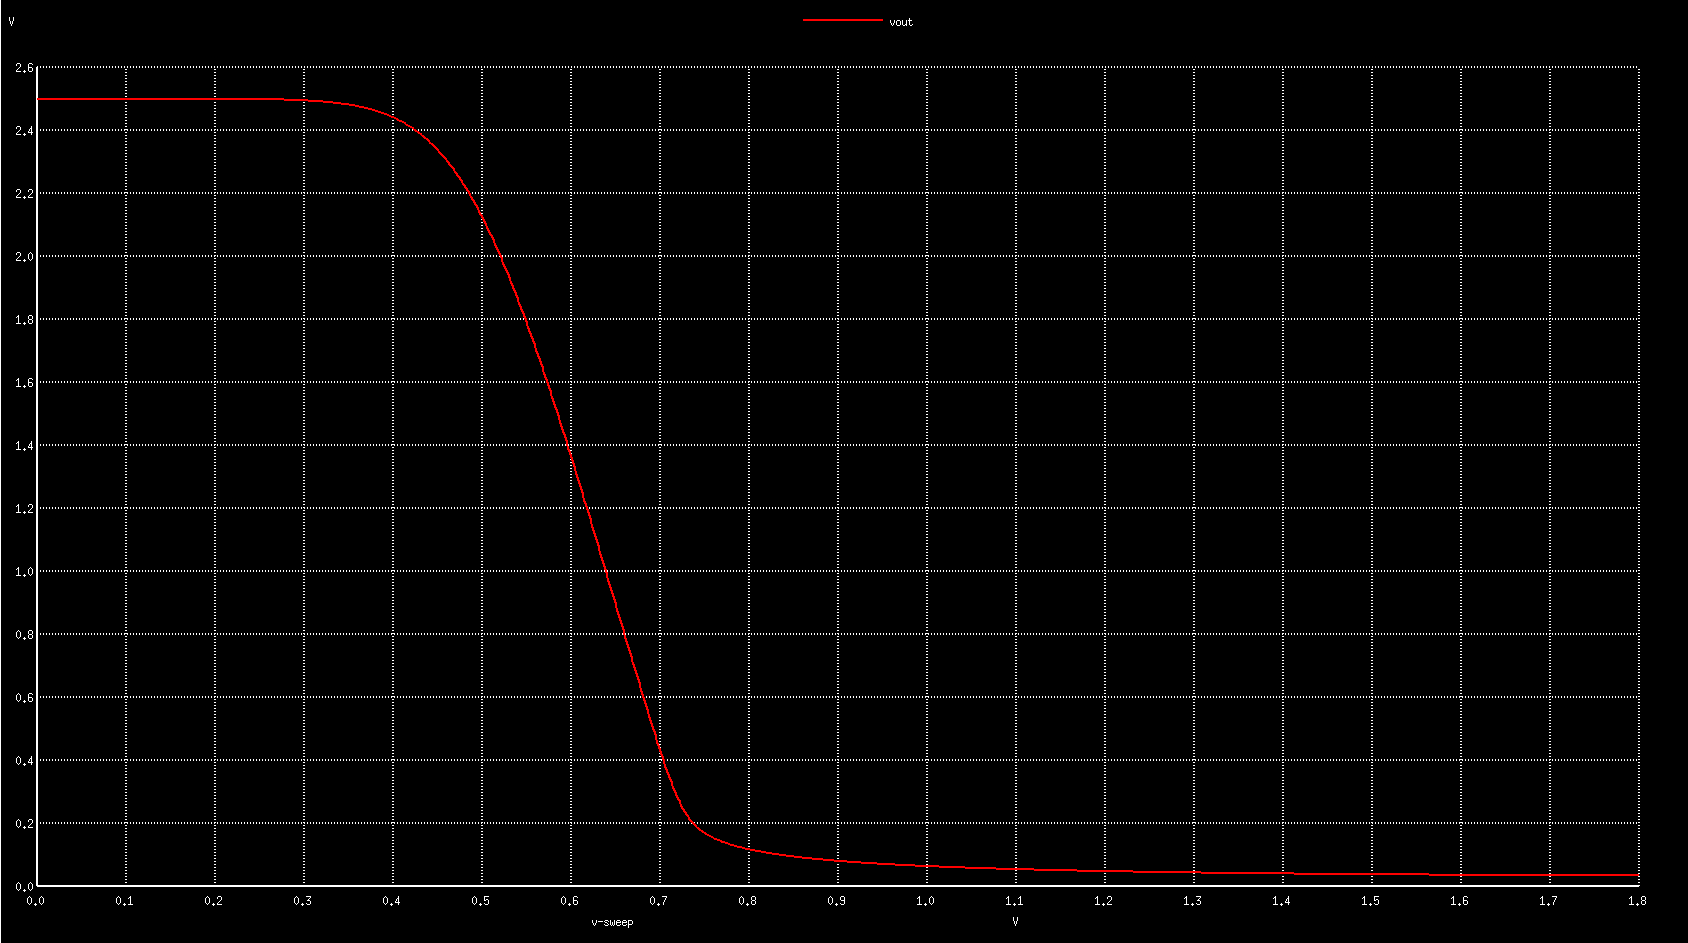
\includegraphics[scale=0.3]{Images/5avtc.png}
    \caption{VT Characteristics}
\end{figure}
\begin{figure}[!ht]
    \centering
    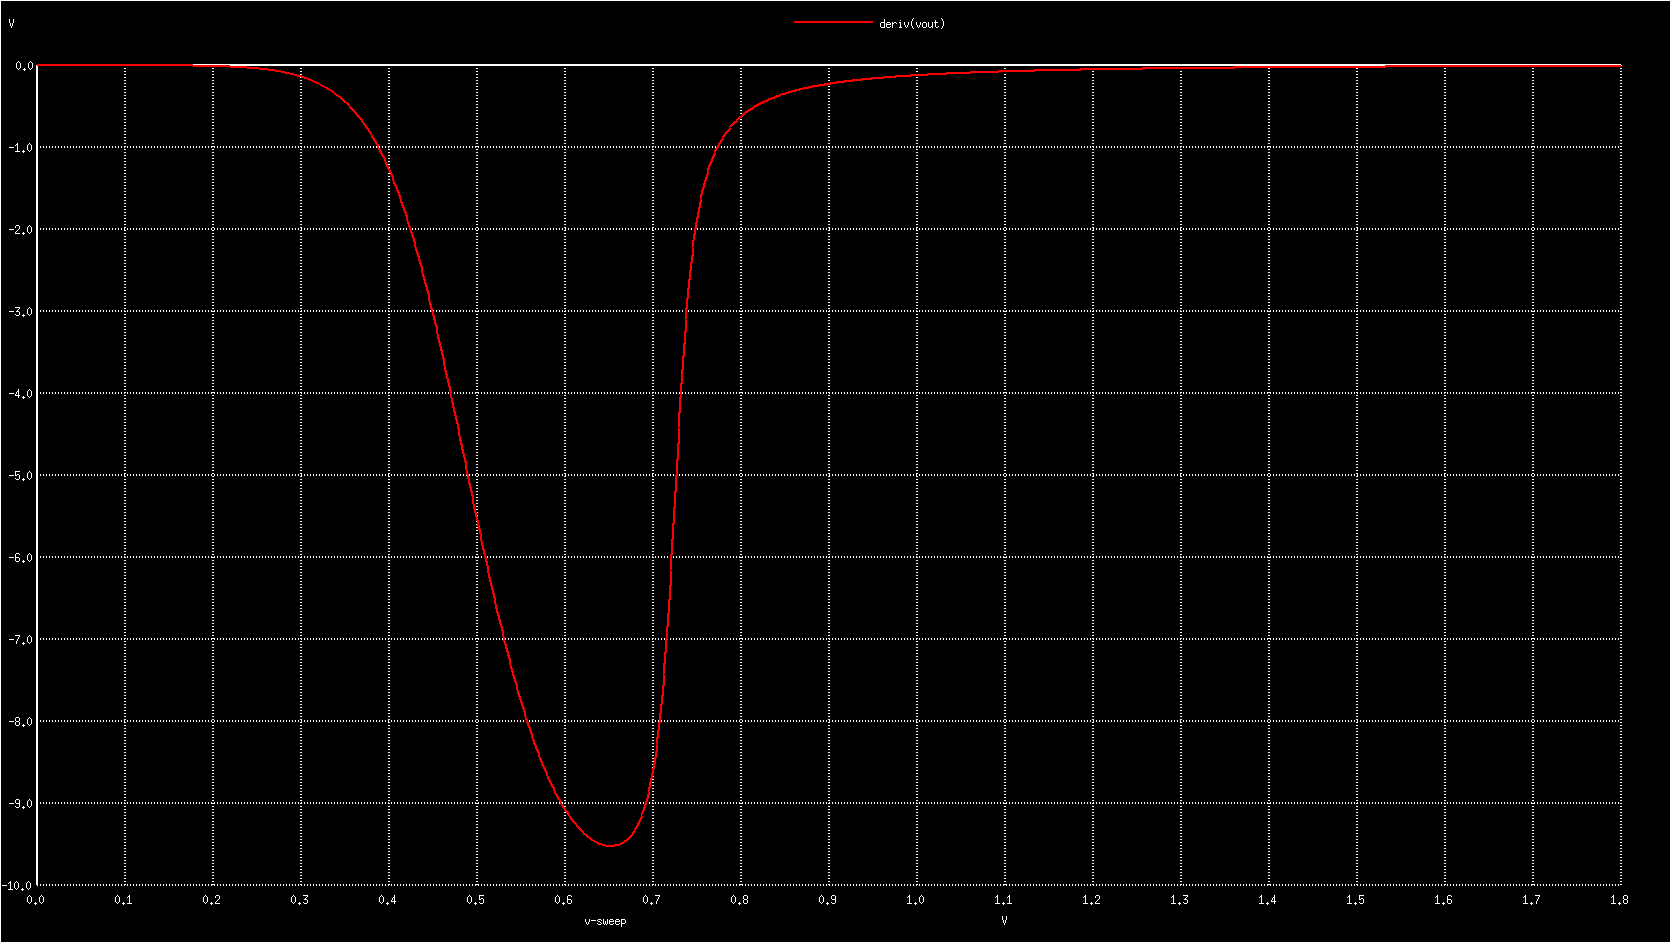
\includegraphics[scale=0.3]{Images/5ar.png}
    \caption{Gain of Inverter}
\end{figure}

\subsection{5b}
As Load Resistance increases Magnitude of Gain Increases. On solving Small Signal Model of MOSFET,
\begin{align}
    \frac{dV_{out}}{dV_{in}} = -g_{m}R_{load}\\
    g_{m} = \mu_nC_{ox}\frac{W}{L}(V_{GS} - V_{Th})
\end{align}
\textbf{SPICE Netlist:}
\begin{lstlisting}
Question-5b
*Load Resistance is varies from 10k to 100k as steps of 10k*

* Model
.include "TSMC180.lib"
.model nch_tt nmos

* Circuit
VG	G	0	1.8
M	D	G	0	0	nch_tt W=540n L=180n
R	D	2	100k
V	2	0	DC	2.5

* Analysis
.dc VG 0 1.8 1m

* Results
.control
run 
let ID = -V#branch
let Vout = V(D)
let Vin = V(G)
*plot	Vout
plot	deriv(Vout) vs V(G)
wrdata ../Data/5b/10.dat		V(G)	deriv(Vout)
.endc

.end
\end{lstlisting}
\textbf{Python Code for Plotting}
\begin{lstlisting}[language=Python]
import numpy as np
import matplotlib.pyplot as plt
import os
def File2Numpy(Path):
	Content = []
	for i in open(Path).readlines():
		Content.append(i.strip().split())
	Content = np.array(Content).astype(float)
	x = Content[:,1]
	y = Content[:,3]
	return np.array([x,y]).T
	
Path = "../Data/5b/"
DataFiles = len(os.listdir(Path))
# Load Resistance
R = np.arange(10,110,10) * 1000
# Gain
Gain, PeakGain, Vm = [], [], []
# Reading Files
for i in range(DataFiles):
	Gain.append(File2Numpy(Path+str(i+1)+".dat"))
Gain = np.array(Gain)
# Plotting Gain as function VG
plt.figure(figsize=(7,7))
for i in range(Gain.shape[0]):
	PeakGain.append(np.min(Gain[i,:,1]))
	ind = np.argmin(Gain[i,:,1])
	Vm.append(Gain[i,ind,0])
	plt.plot(Gain[i,:,0],Gain[i,:,1], label=str(int(R[i]/1000))+"K ohm")
plt.legend()
plt.grid()
plt.title(r"Gain vs $V_G$")
plt.xlabel(r"$V_G$")
plt.ylabel("Gain")
plt.savefig("5b_Gain.png")
# Plotting Peak Gain
plt.figure(figsize=(7,7))
plt.plot(R,PeakGain)
plt.grid()
plt.title(r"PeakGain vs R")
plt.xlabel("R")
plt.ylabel("PeakGain")
plt.savefig("5b_PeakGain.png")
# Plotting Vm
plt.figure(figsize=(7,7))
plt.plot(R,Vm)
plt.grid()
plt.title(r"Vm vs R")
plt.xlabel("R")
plt.ylabel("Vm")
plt.savefig("5b_Vm.png")
plt.show()
\end{lstlisting}
\textbf{Results:}
\begin{figure}[!ht]
    \centering
    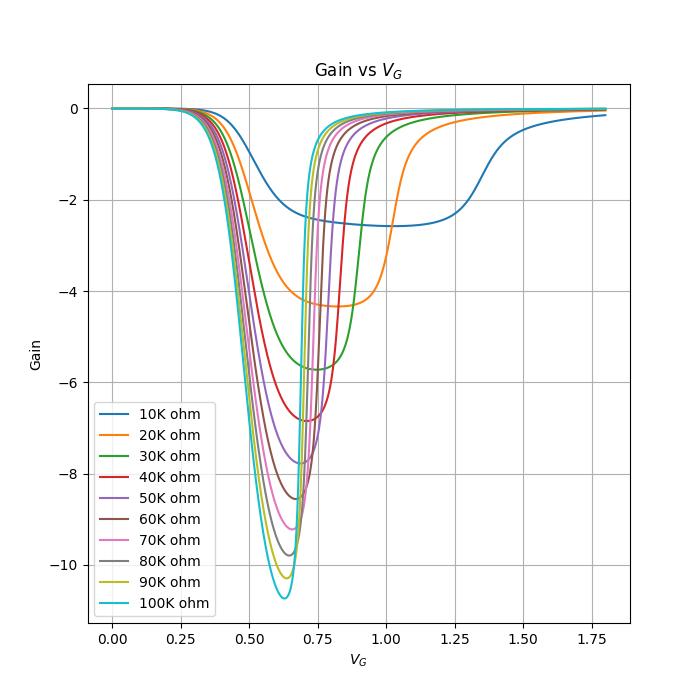
\includegraphics[scale=0.75]{Images/5b_Gain.png}
    \caption{Gain vs $V_G$}
\end{figure}
\begin{figure}[!ht]
    \centering
    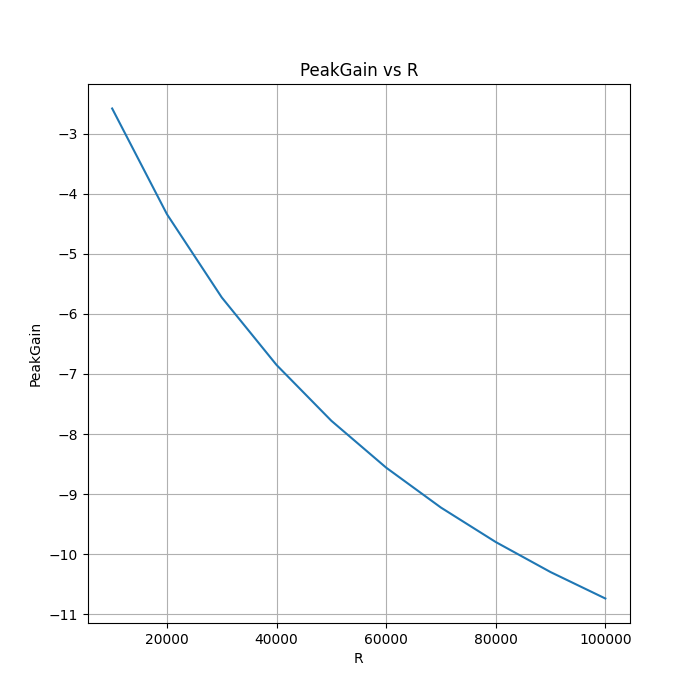
\includegraphics[scale=0.5]{Images/5b_PeakGain.png}
    \caption{Peak Gain vs $R_{load}$}
\end{figure}
\begin{figure}[!ht]
    \centering
    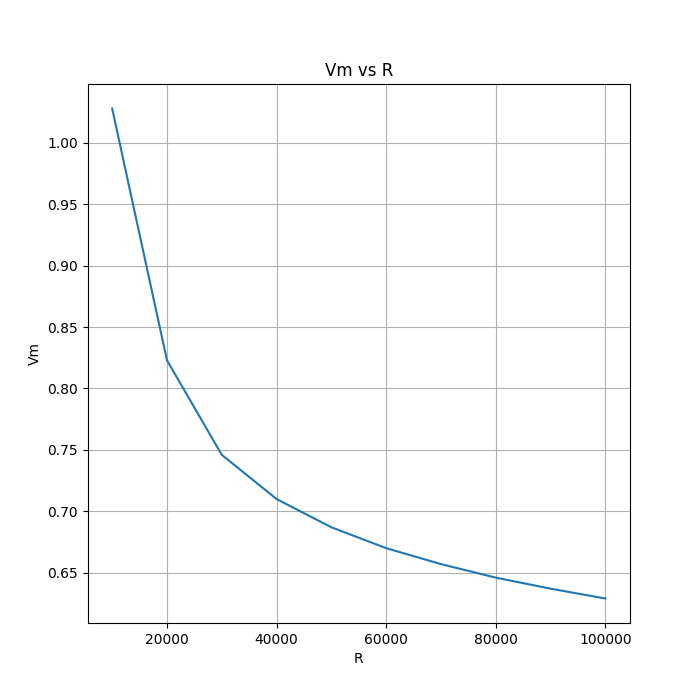
\includegraphics[scale=0.5]{Images/5b_Vm.png}
    \caption{$V_m$ vs $R_{load}$}
\end{figure}
\subsection{5c}
\begin{align}
    C = 3pF
\end{align}
\textbf{SPICE Netlist}
\begin{lstlisting}
Question-5c

* Model
.include "TSMC180.lib"
.model nch_tt nmos

* Circuit
VG	G	0	PULSE(0 1 0 0 0 2u 4u)
M	D	G	0	0	nch_tt W=540n L=180n
R	D	2	75k
V	2	0	DC	2.5
C	D	0	3p

* Analysis
.tran	0.1n	10u

* Results
.control
run 
let ID = -V#branch
let Vout = V(D)
let Vin = V(G)
plot	Vin
plot	Vout
.endc

.end
\end{lstlisting}
\textbf{Results:}
\begin{figure}[!ht]
    \centering
    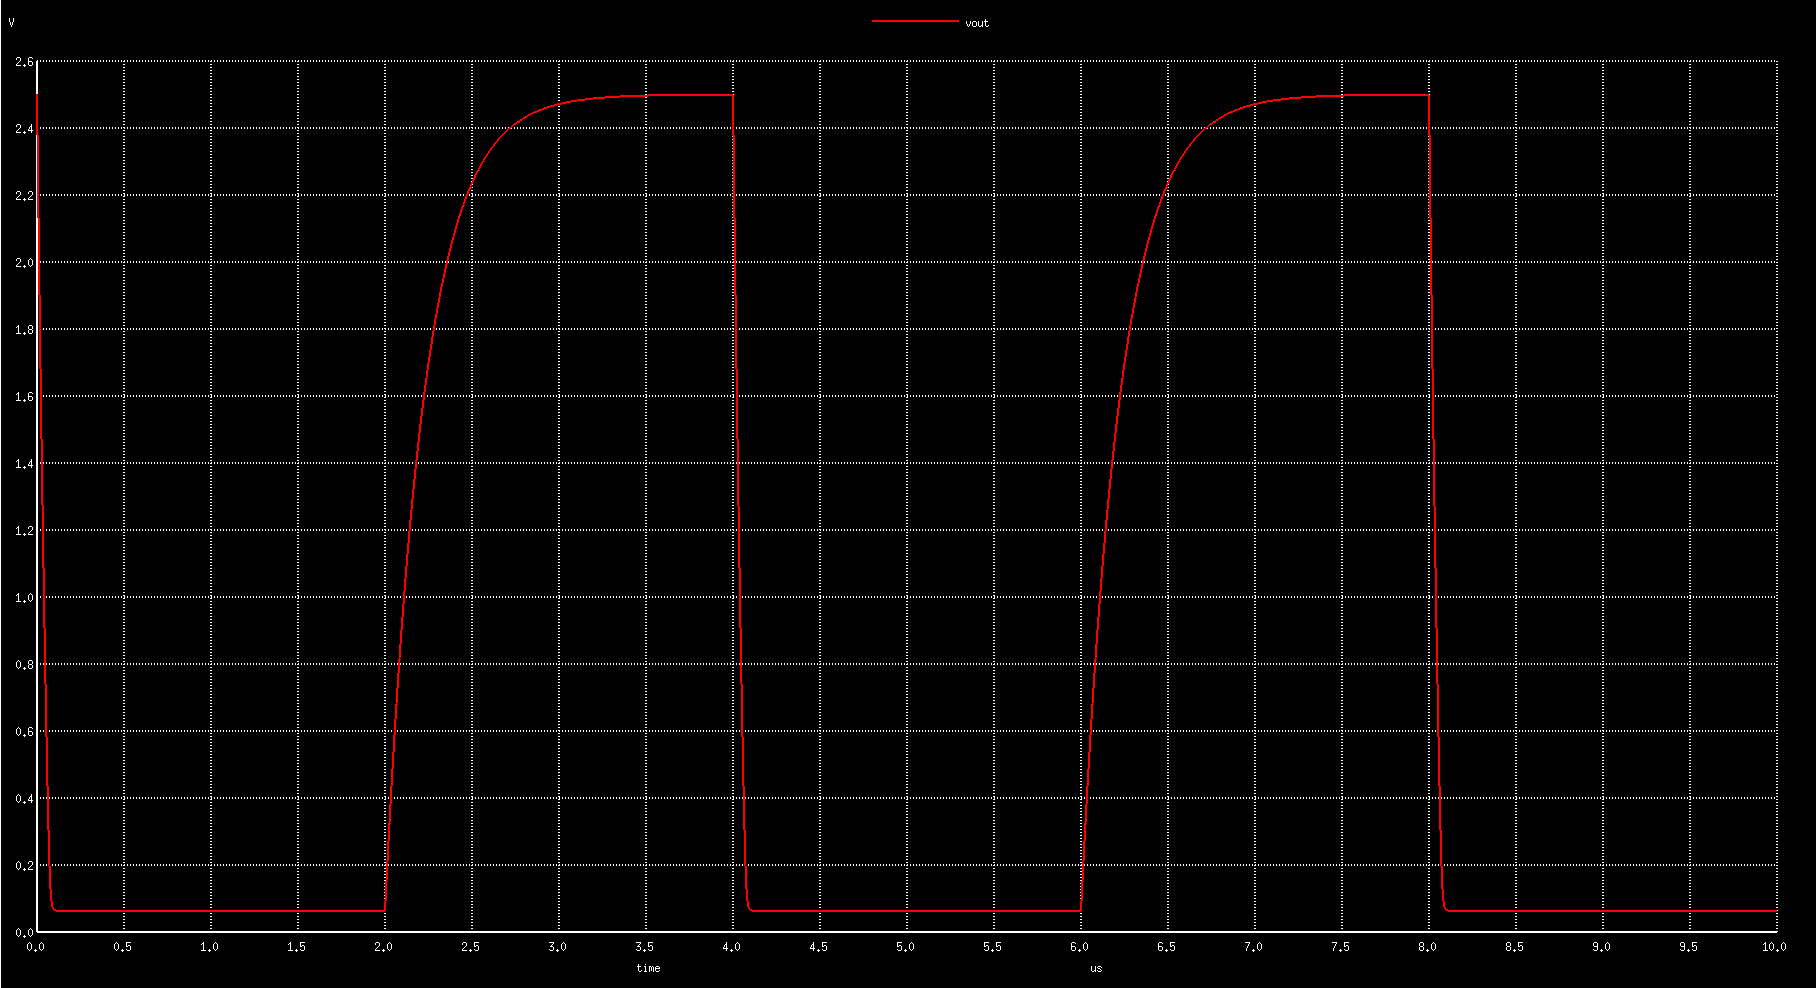
\includegraphics[scale=0.25]{Images/5coutput.png}
    \caption{Output of the Circuit for an Ideal Clock Signal with $f=250k\text{Hz}$ and duty-cycle of 50\%}
\end{figure}
\begin{align}
    t_r = 0.489 \text{ $\mu$s}\\
    t_p = 32.0896 \text{ ns}\\
    t_f = 63.134 \text{ ns}
\end{align}
Rise Time and Fall Time are difference is due to the Resistance of MOSFET. During Rise Time of $V_{out}$, $V_{in} = low$, which means MOSFET is turned off. So, Capacitor gets charged by drawing Power through Resistor($R_L$) from $V_{DD}$. When discharging i.e during Fall of Output, Capacitors gets discharged through MOSFET and due to Low Resistance of MOSFET when compared to $R_{L}$, Fall-Time is less than Rise-Time of Output.
\end{document}
